
\newpage
\section{Theoretical Analysis}
\label{sec:analysis}

Solvig the OP problem we get $VCE=2.1578$

Regarding the gains plots between the first and 2 stage we can see that they do not differ alot, this is beliveble since AV2=-0.0348 db as we can see in the table, so it does not vary much the result.


\begin{figure}[h]
\centering
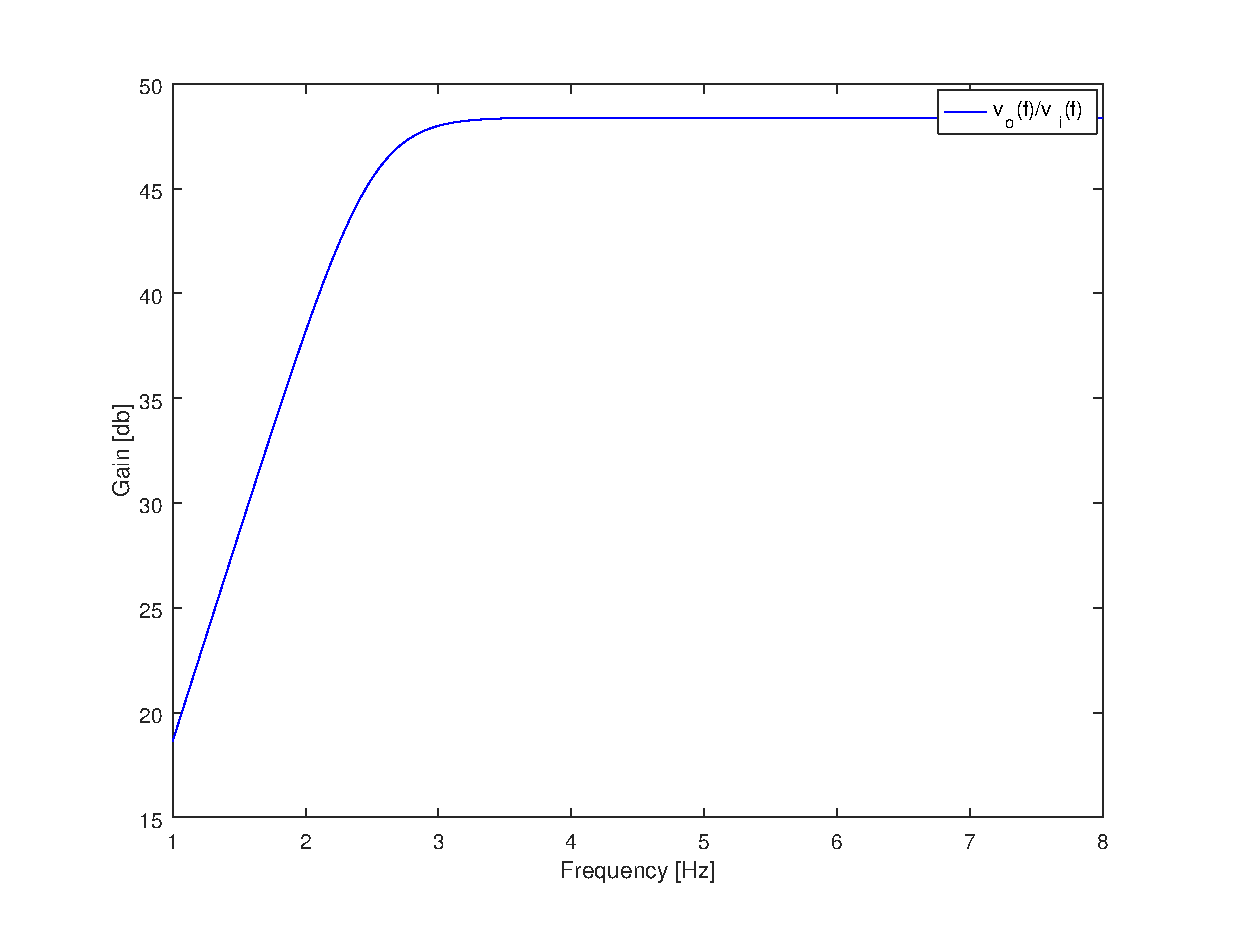
\includegraphics[width=0.6\linewidth]{Gain1.eps}
\caption{Gain in the first phase}
\label{plot:ganho1}
\end{figure}


Nevertheless the inputs and outputs for this stages are present in the following table:


\begin{table}[h]
\begin{tabular}{ll}
AV1 & 262.79 \\
ZI1 & 484.43 \\
Z01 & 886.28 \\
AV2 & 0.996  \\
ZI2 & 8598.9 \\
Z02 & 0.302 
\end{tabular}
\end{table}

\newpage

As such the final gain plot can be given by the following Figure.
\begin{figure}[h]
\centering
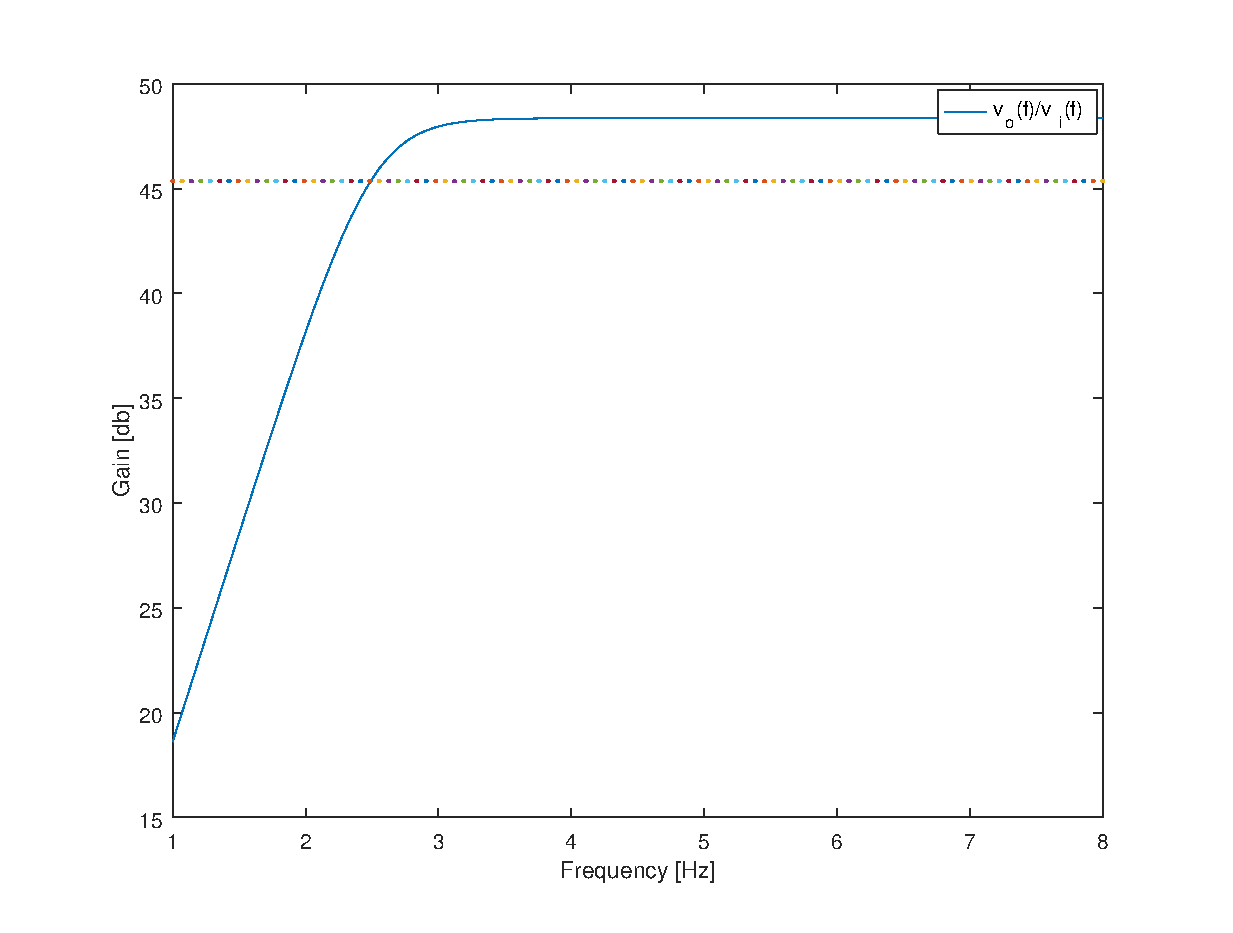
\includegraphics[width=0.6\linewidth]{GainFinal.eps}
\caption{Output Gain}
\label{plot:ganho2}
\end{figure}


